\documentclass[aspectratio=169,handout]{beamer}
% \usepackage[utf8]{inputenc}
\usetheme{metropolis}
\usecolortheme{orchid}
\usepackage{amsmath}
\usepackage{amssymb}
\usepackage{amsthm}
\usepackage{multirow}
\usepackage[ruled]{algorithm2e}
\usepackage{mathtools}
\usepackage{caption}
% \usepackage{epstopdf}
\usepackage{hyperref}
\usepackage{subcaption}
\usepackage{siunitx}
\usepackage{textcomp}
\usepackage{tcolorbox}
\usepackage{tikz}
\usetikzlibrary{mindmap,shadows,tikzmark,positioning,arrows.meta,shapes.misc}

\setbeamerfont{footnote}{size=\tiny}

% Information boxes
\newcommand*{\info}[4][16.3]{%
  \node [ annotation, #3, scale=0.65, text width = #1em,
          inner sep = 2mm ] at (#2) {%
  \list{$\bullet$}{\topsep=0pt\itemsep=0pt\parsep=0pt
    \parskip=0pt\labelwidth=8pt\leftmargin=8pt
    \itemindent=0pt\labelsep=2pt}%
    #4
  \endlist
  };
}

%% Definitions for root locus plots
\newcommand*{\rootlocusexample}[2]{% ymin,ymax,
		\foreach \x in {-4,-3,-2,-1}
   		\draw (\x cm,1pt) -- (\x cm,-1pt) node[anchor=north] {$\x$};
		\foreach \y in {-1,1}
   		\draw (-1pt,\y cm) -- (1pt,\y cm) node[anchor=east] {$\y$};
		\draw [-latex] (-4.5,0) -- (1,0) node [above]  {$\sigma$};
		\draw [-latex] (0,#1) -- (0,#2) node [right] {$j\omega$};
		\node[pole,draw=black] at (0,0) {};
		\node[pole,draw=black] at (-1,0) {};
		\node[pole,draw=black] at (-2,0) {};
		\node[zero,draw=black] at (-3,0) {};
		\node[pole,draw=black] at (-4,0) {};
}

\tikzset{%
  >={Latex[width=2mm,length=2mm]},
  % Specifications for style of nodes:
            base/.style = {rectangle, rounded corners, draw=black,
                           minimum width=4cm, minimum height=1cm,
                           text centered, font=\sffamily},
  activityStarts/.style = {base, fill=blue!30},
       startstop/.style = {base, fill=red!30},
    activityRuns/.style = {base, fill=green!30},
         process/.style = {base, minimum width=2.5cm, fill=orange!15,
                           font=\ttfamily},
}

\tikzset{pole/.style={cross out, draw=black, minimum size=2*(#1-\pgflinewidth), inner sep=0pt, outer sep=0pt},
pole/.default={3pt}}
\tikzset{zero/.style={circle, draw=black, fill=white, minimum size=2*(#1-\pgflinewidth), inner sep=0pt, outer sep=0pt},
zero/.default={3pt}}
\tikzset{test/.style={rectangle, draw=black, fill=white, minimum size=2*(#1-\pgflinewidth), inner sep=0pt, outer sep=0pt},
test/.default={3pt}}

%% Definitions for block diagrams
\tikzstyle{block} = [draw, fill=blue!20, rectangle, 
    minimum height=2em, minimum width=3em]
\tikzstyle{sum} = [draw, fill=blue!20, circle, node distance=1cm]
\tikzstyle{input} = [coordinate]
\tikzstyle{output} = [coordinate]
\tikzstyle{pinstyle} = [pin edge={to-,thin,black}]

\renewcommand\textbullet{\ensuremath{\bullet}}
\newcommand\scalemath[2]{\scalebox{#1}{\mbox{\ensuremath{\displaystyle #2}}}}
\newcommand{\norm}[1]{\left\lVert#1\right\rVert}

%%% Bibliography
\usepackage[citestyle=numeric,style=numeric,backend=biber,doi=false,isbn=false,url=false]{biblatex}
\addbibresource{references.bib}

%%% Suppress biblatex annoying warning
\usepackage{silence}
\WarningFilter{biblatex}{Patching footnotes failed}

%%% new theorems %%%%%%%%%%%%%%%%%%%%%%%%%%%%%%%%%%%%%%%%%%%%%%%%%%%%%%%%%%%%%%
\theoremstyle{definition}
\newtheorem{mydef}{Definition}

\theoremstyle{plain}
\newtheorem{mylemma}{Lemma}[section]
\newtheorem{mytheorem}{Theorem}[section]
\newtheorem{myproposition}{Proposition}[section]
\newtheorem{myproblem}{Problem}[section]
\newtheorem{mydefinition}{Definition}[section]
\newtheorem{myassumption}{Assumption}[section]

\theoremstyle{remark}
\newtheorem{myremark}{Remark}[section]

\newcounter{saveenumi}
\newcommand{\seti}{\setcounter{saveenumi}{\value{enumi}}}
\newcommand{\conti}{\setcounter{enumi}{\value{saveenumi}}}

\resetcounteronoverlays{saveenumi}

\title{Controles}
\subtitle{\small Clase 6: Diseño de Compensadores por LGR - Aproximación de Polos Dominantes}
\author{Gerardo Becerra, Ph.D.}
\institute{Pontificia Universidad Javeriana\\ Departamento de Electrónica}
\date{Marzo 4, 2020}

\begin{document}

\frame{\titlepage}	

\begin{frame}[<+->]\frametitle{Introducción}
\vspace*{5mm}
\centering
\begin{itemize}
	\item Estabilidad y desempeño de un sistema de control retroalimentado $\rightarrow$ dependen de la ubicación de los polos de lazo cerrado en el plano complejo.
	\item Es interesante determinar cómo se mueven las raíces del polinomio característico a medida que se modifican ciertos parámetros $\rightarrow$ lugar de las raíces.
	\item Método de lugar de las raíces: método gráfico para hacer un bosquejo del lugar de las raíces.
	\item Información gráfica $\rightarrow$ información cualitativa de la estabilidad y desempeño del sistema.
	\item Es posible usar el lugar de las raíces para diseñar controladores.
\end{itemize}
\end{frame}

\section{Método del Lugar de las Raíces}
\begin{frame}[<+->]\frametitle{Método del Lugar de las Raíces}
	\begin{figure}
		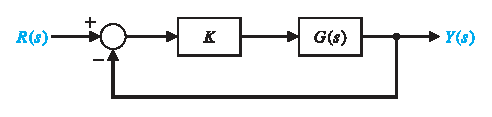
\includegraphics[width=6cm]{images/controlsystem.eps}
	\end{figure}
	\vspace*{-3mm}
	\begin{columns}
	\begin{column}{0.5\textwidth}
	\begin{itemize}
		\item El comportamiento dinámico del sistema de control se describe por la función de transferencia
		\begin{equation*}
			T(s) = \frac{Y(s)}{R(s)} = \frac{p(s)}{q(s)}
		\end{equation*}
		\item El polinomio característico para el sistema de control de la figura es:
		\begin{equation*}
			1 + K G(s) = 0,\hspace*{3mm} 0 \leq K < \infty
		\end{equation*}
	\end{itemize}
	\end{column}	
	\begin{column}{0.5\textwidth}
	\begin{itemize}
		\item La ecuación se puede reescribir en forma polar como
		\begin{equation*}
			|KG(s)| \angle KG(s) = -1 + j0
		\end{equation*}
		\item Por lo tanto se debe cumplir
		\begin{align*}
			|KG(s)| &= 1\\
			\angle KG(s) &= 180^o + k360^o
		\end{align*}
	\end{itemize}
	\end{column}	
	\end{columns}
\end{frame}

\begin{frame}[<+->]\frametitle{Método del Lugar de las Raíces}
	\begin{itemize}
		\item El LGR debe satisfacer la condición de magnitud:
		\begin{equation*}
			|KG(s)| = \frac{K|s+z_1||s+z_2|\dots|s+z_M|}{|s+p_1||s+p_2|\dots|s+p_n|} = 1
		\end{equation*}
		y la condición de ángulo:
		\begin{equation*}
			\angle G(s) = \sum_{i=1}^M \angle(s+z_i) - \sum_{j=1}^n \angle(s+p_j) = 180^o + k360^o 
		\end{equation*}
	\end{itemize}
\end{frame}

\begin{frame}[c]\frametitle{Método del Lugar de las Raíces}
	\centering
	\textbf{El lugar de las raíces corresponde a las trayectorias seguidas por las raíces de la ecuación característica a medida que un parámetro del sistema varía desde cero hasta infinito.}
\end{frame}

\section{Lugar de las Raíces - Procedimiento}

\begin{frame}[<+->]\frametitle{Paso 1: Preparar el diagrama}
\small
\begin{columns}
	\begin{column}{0.5\textwidth}
	\begin{itemize}
		\item Escribir la ecuación característica para que el parámetro de interés $K$ aparezca como un factor multiplicativo
		\begin{equation*}
			1 + KG(s) = 0
		\end{equation*}
		\item Factorizar $G(s)$ y escribir el polinomio en la forma de polos y ceros:
		\begin{equation}
			1 + K \frac{\prod_{i=1}^M (s + z_i)}{\prod_{j=1}^n (s + p_j)}
			\label{eq:PolesandZerosinCharacteristicPolynomial}
		\end{equation}
	\end{itemize}
	\end{column}
	\begin{column}{0.5\textwidth}
	\begin{itemize}
		\item Localice los ceros $-z_i$ y polos $-p_j$ en el plano complejo usando los símbolos $\times$ y $\bigcirc$, respectivamente.
		\item Reescribiendo la Eq.\eqref{eq:PolesandZerosinCharacteristicPolynomial} se tiene:
		\begin{align*}
			\prod_{j=1}^n (s + p_j) + K \prod_{i=1}^n (s + z_j) &= 0\\
			\frac{1}{K}\prod_{j=1}^n (s + p_j) + \prod_{i=1}^n (s + z_j) &= 0
		\end{align*}
		\pause
		Si $K = 0$ $\Rightarrow$ las raíces del polinomio característico son los polos de $G(s)$.\\
		\pause
		Si $K \rightarrow \infty$ $\Rightarrow$ las raíces del polinomio característico son los ceros de $G(s)$.
	\end{itemize}
	\end{column}
\end{columns}
\end{frame}

\begin{frame}[c]\frametitle{Paso 1: Preparar el diagrama}
	\textbf{El lugar de las raíces de la ecuación característica $1 + KG(s)= 0$ inicia en los polos de $G(s)$ y termina en los ceros de $G(s)$ a medida que $K$ se incrementa desde cero hasta infinito.}
\end{frame}

\begin{frame}[<+->]\frametitle{Paso 1 - Ejemplo}
\begin{columns}
	\begin{column}{0.5\textwidth}
		\begin{equation*}
			G(s) = \frac{(s+3)}{s(s+1)(s+2)(s+4)}
		\end{equation*}
	\end{column}
	\begin{column}{0.5\textwidth}
	\begin{tikzpicture}
		\rootlocusexample{-2}{2}
		% \foreach \x in {-4,-3,-2,-1}
  %  		\draw (\x cm,1pt) -- (\x cm,-1pt) node[anchor=north] {$\x$};
		% \draw [-latex] (-5,0) -- (1,0) node [above]  {$\sigma$};
		% \draw [-latex] (0,-2) -- (0,2) node [right] {$j\omega$};
		% \node[pole,draw=black] at (0,0) {};
		% \node[pole,draw=black] at (-1,0) {};
		% \node[pole,draw=black] at (-2,0) {};
		% \node[zero,draw=black] at (-3,0) {};
		% \node[pole,draw=black] at (-4,0) {};
	\end{tikzpicture}
	\centering
	Ubicación de polos y ceros del sistema en lazo abierto.
	\end{column}
\end{columns}
\end{frame}

\begin{frame}[c]\frametitle{Paso 2: Localizar segmentos del LGR en el eje real}
\centering
\textbf{Usando la condición de ángulo es posible determinar los segmentos del eje real que hacen parte del lugar de las raíces.}
\end{frame}

\begin{frame}[c]\frametitle{Paso 2: Localizar segmentos del LGR en el eje real - Ejemplo}
Condición de ángulo en el intervalo $[-1,0]$
\begin{figure}
	\vspace*{0.5cm}
	\centering
	\begin{minipage}[b]{.5\linewidth}
		\centering	
		\begin{tikzpicture}[transform canvas={scale=0.9}]
			\rootlocusexample{-1.2}{1.2}
			\node[test,draw=black] at (-0.5,0) {};
			\draw [->, line width=2pt, red] (0,0) -- (-0.5,0) {};
			\draw [red, -stealth] (0.2,0) arc (0:180:0.2);
			\draw [->, line width=2pt, blue] (-1,0) -- (-0.5,0) {};
		\end{tikzpicture}
	\end{minipage}%
	\begin{minipage}[b]{.5\linewidth}
	\centering
		\begin{tikzpicture}[transform canvas={scale=0.9}]
			\rootlocusexample{-1.2}{1.2}
			\node[test,draw=black] at (-0.5,0) {};
			\draw [->, line width=2pt, green] (-2,0) -- (-0.5,0) {};
		\end{tikzpicture}
	\end{minipage}\\
	\vspace*{2cm}
	\begin{minipage}[b]{.5\linewidth}
	\centering
		\begin{tikzpicture}[transform canvas={scale=0.9}]
			\rootlocusexample{-1.2}{1.2}
			\node[test,draw=black] at (-0.5,0) {};
			\draw [->, line width=2pt, cyan] (-3,0) -- (-0.5,0) {};
		\end{tikzpicture}
	\end{minipage}%
	\begin{minipage}[b]{.5\linewidth}
	\centering
		\begin{tikzpicture}[transform canvas={scale=0.9}]
			\rootlocusexample{-1.2}{1.2}
			\node[test,draw=black] at (-0.5,0) {};
			\draw [->, line width=2pt, magenta] (-4,0) -- (-0.5,0) {};
		\end{tikzpicture}
	\end{minipage}
\end{figure}
\vspace*{5mm}
\begin{align*}
	&\textcolor{cyan}{\angle(s+3)} - \left(\textcolor{red}{\angle(s)} + \textcolor{blue}{\angle(s+1)} + \textcolor{green}{\angle(s+2)} + \textcolor{magenta}{\angle(s+4)}\right)\\
	&= \textcolor{cyan}{\ang{0}} - \left(\textcolor{red}{\ang{180}} + \textcolor{blue}{\ang{0}} + \textcolor{green}{\ang{0}} + \textcolor{magenta}{\ang{0}}\right) = -\ang{180} \Rightarrow \text{El segmento si pertenece al LGR.}
\end{align*}
\end{frame}

\begin{frame}[c]\frametitle{Paso 2: Localizar segmentos del LGR en el eje real - Ejemplo}
Condición de ángulo en el intervalo $[-2,-1]$
\begin{figure}
	\vspace*{0.5cm}
	\centering
	\begin{minipage}[b]{.5\linewidth}
		\centering	
		\begin{tikzpicture}[transform canvas={scale=0.9}]
			\rootlocusexample{-1.2}{1.2}
			\node[test,draw=black] at (-1.5,0) {};
			\draw [->, line width=2pt, red] (0,0) -- (-1.5,0) {};
			\draw [red, -stealth] (0.5,0) arc (0:180:0.5);
		\end{tikzpicture}
	\end{minipage}%
	\begin{minipage}[b]{.5\linewidth}
	\centering
		\begin{tikzpicture}[transform canvas={scale=0.9}]
			\rootlocusexample{-1.2}{1.2}
			\node[test,draw=black] at (-1.5,0) {};
			\draw [->, line width=2pt, blue] (-1,0) -- (-1.5,0) {};
			\draw [blue, -stealth] (-0.8,0) arc (0:180:0.2);
			\draw [->, line width=2pt, green] (-2,0) -- (-1.5,0) {};
		\end{tikzpicture}
	\end{minipage}\\
	\vspace*{2cm}
	\begin{minipage}[b]{.5\linewidth}
	\centering
		\begin{tikzpicture}[transform canvas={scale=0.9}]
			\rootlocusexample{-1.2}{1.2}
			\node[test,draw=black] at (-1.5,0) {};
			\draw [->, line width=2pt, cyan] (-3,0) -- (-1.5,0) {};
		\end{tikzpicture}
	\end{minipage}%
	\begin{minipage}[b]{.5\linewidth}
	\centering
		\begin{tikzpicture}[transform canvas={scale=0.9}]
			\rootlocusexample{-1.2}{1.2}
			\node[test,draw=black] at (-1.5,0) {};
			\draw [->, line width=2pt, magenta] (-4,0) -- (-1.5,0) {};
		\end{tikzpicture}
	\end{minipage}
\end{figure}
\vspace*{5mm}
\begin{align*}
	&\textcolor{cyan}{\angle(s+3)} - \left(\textcolor{red}{\angle(s)} + \textcolor{blue}{\angle(s+1)} + \textcolor{green}{\angle(s+2)} + \textcolor{magenta}{\angle(s+4)}\right)\\
	&= \textcolor{cyan}{\ang{0}} - \left(\textcolor{red}{\ang{180}} + \textcolor{blue}{\ang{180}} + \textcolor{green}{\ang{0}} + \textcolor{magenta}{\ang{0}}\right) = -\ang{360} \neq 180 \Rightarrow \text{El segmento no pertenece al LGR.}
\end{align*}
\end{frame}

\begin{frame}[c]\frametitle{Paso 2: Localizar segmentos del LGR en el eje real - Ejemplo}
Condición de ángulo en el intervalo $[-3,-2]$
\begin{figure}
	\vspace*{0.5cm}
	\centering
	\begin{minipage}[b]{.5\linewidth}
		\centering	
		\begin{tikzpicture}[transform canvas={scale=0.9}]
			\rootlocusexample{-1.2}{1.2}
			\node[test,draw=black] at (-2.5,0) {};
			\draw [->, line width=2pt, red] (0,0) -- (-2.5,0) {};
			\draw [red, -stealth] (0.5,0) arc (0:180:0.5);
		\end{tikzpicture}
	\end{minipage}%
	\begin{minipage}[b]{.5\linewidth}
	\centering
		\begin{tikzpicture}[transform canvas={scale=0.9}]
			\rootlocusexample{-1.2}{1.2}
			\node[test,draw=black] at (-2.5,0) {};
			\draw [->, line width=2pt, blue] (-1,0) -- (-2.5,0) {};
			\draw [blue, -stealth] (-0.5,0) arc (0:180:0.5);
		\end{tikzpicture}
	\end{minipage}\\
	\vspace*{2cm}
	\begin{minipage}[b]{.5\linewidth}
	\centering
		\begin{tikzpicture}[transform canvas={scale=0.9}]
			\rootlocusexample{-1.2}{1.2}
			\node[test,draw=black] at (-2.5,0) {};
			\draw [->, line width=2pt, green] (-2,0) -- (-2.5,0) {};
			\draw [green, -stealth] (-1.8,0) arc (0:180:0.2);
			\draw [->, line width=2pt, cyan] (-3,0) -- (-2.5,0) {};
		\end{tikzpicture}
	\end{minipage}%
	\begin{minipage}[b]{.5\linewidth}
	\centering
		\begin{tikzpicture}[transform canvas={scale=0.9}]
			\rootlocusexample{-1.2}{1.2}
			\node[test,draw=black] at (-2.5,0) {};
			\draw [->, line width=2pt, magenta] (-4,0) -- (-2.5,0) {};
		\end{tikzpicture}
	\end{minipage}
\end{figure}
\vspace*{5mm}
\begin{align*}
	&\textcolor{cyan}{\angle(s+3)} - \left(\textcolor{red}{\angle(s)} + \textcolor{blue}{\angle(s+1)} + \textcolor{green}{\angle(s+2)} + \textcolor{magenta}{\angle(s+4)}\right)\\
	&= \textcolor{cyan}{\ang{0}} - \left(\textcolor{red}{\ang{180}} + \textcolor{blue}{\ang{180}} + \textcolor{green}{\ang{180}} + \textcolor{magenta}{\ang{0}}\right) = -180 \Rightarrow \text{El segmento si pertenece al LGR.}
\end{align*}
\end{frame}

\begin{frame}[c]\frametitle{Paso 2: Localizar segmentos del LGR en el eje real - Ejemplo}
Condición de ángulo en el intervalo $[-4,-3]$
\begin{figure}
	\vspace*{0.5cm}
	\centering
	\begin{minipage}[b]{.5\linewidth}
		\centering	
		\begin{tikzpicture}[transform canvas={scale=0.9}]
			\rootlocusexample{-1.2}{1.2}
			\node[test,draw=black] at (-3.5,0) {};
			\draw [->, line width=2pt, red] (0,0) -- (-3.5,0) {};
			\draw [red, -stealth] (0.5,0) arc (0:180:0.5);
		\end{tikzpicture}
	\end{minipage}%
	\begin{minipage}[b]{.5\linewidth}
	\centering
		\begin{tikzpicture}[transform canvas={scale=0.9}]
			\rootlocusexample{-1.2}{1.2}
			\node[test,draw=black] at (-3.5,0) {};
			\draw [->, line width=2pt, blue] (-1,0) -- (-3.5,0) {};
			\draw [blue, -stealth] (-0.5,0) arc (0:180:0.5);
		\end{tikzpicture}
	\end{minipage}\\
	\vspace*{2cm}
	\begin{minipage}[b]{.5\linewidth}
	\centering
		\begin{tikzpicture}[transform canvas={scale=0.9}]
			\rootlocusexample{-1.2}{1.2}
			\node[test,draw=black] at (-3.5,0) {};
			\draw [->, line width=2pt, green] (-2,0) -- (-3.5,0) {};
			\draw [green, -stealth] (-1.5,0) arc (0:180:0.5);
		\end{tikzpicture}
	\end{minipage}%
	\begin{minipage}[b]{.5\linewidth}
	\centering
		\begin{tikzpicture}[transform canvas={scale=0.9}]
			\rootlocusexample{-1.2}{1.2}
			\node[test,draw=black] at (-3.5,0) {};
			\draw [->, line width=2pt, cyan] (-3,0) -- (-3.5,0) {};
			\draw [cyan, -stealth] (-2.8,0) arc (0:180:0.2);
			\draw [->, line width=2pt, magenta] (-4,0) -- (-3.5,0) {};
		\end{tikzpicture}
	\end{minipage}
\end{figure}
\vspace*{5mm}
\begin{align*}
	&\textcolor{cyan}{\angle(s+3)} - \left(\textcolor{red}{\angle(s)} + \textcolor{blue}{\angle(s+1)} + \textcolor{green}{\angle(s+2)} + \textcolor{magenta}{\angle(s+4)}\right)\\
	&= \textcolor{cyan}{\ang{180}} - \left(\textcolor{red}{\ang{180}} + \textcolor{blue}{\ang{180}} + \textcolor{green}{\ang{180}} + \textcolor{magenta}{\ang{0}}\right) = -360 \neq 180\Rightarrow \text{El segmento no pertenece al LGR.}
\end{align*}
\end{frame}

\begin{frame}[c]\frametitle{Paso 2: Localizar segmentos del LGR en el eje real - Ejemplo}
Condición de ángulo en el intervalo $(-\infty,-4]$
\begin{figure}
	\vspace*{0.5cm}
	\centering
	\begin{minipage}[b]{.5\linewidth}
		\centering	
		\begin{tikzpicture}[transform canvas={scale=0.9}]
			\rootlocusexample{-1.2}{1.2}
			\node[test,draw=black] at (-4.5,0) {};
			\draw [->, line width=2pt, red] (0,0) -- (-4.5,0) {};
			\draw [red, -stealth] (0.5,0) arc (0:180:0.5);
		\end{tikzpicture}
	\end{minipage}%
	\begin{minipage}[b]{.5\linewidth}
	\centering
		\begin{tikzpicture}[transform canvas={scale=0.9}]
			\rootlocusexample{-1.2}{1.2}
			\node[test,draw=black] at (-4.5,0) {};
			\draw [->, line width=2pt, blue] (-1,0) -- (-4.5,0) {};
			\draw [blue, -stealth] (-0.5,0) arc (0:180:0.5);
		\end{tikzpicture}
	\end{minipage}\\
	\vspace*{2cm}
	\begin{minipage}[b]{.5\linewidth}
	\centering
		\begin{tikzpicture}[transform canvas={scale=0.9}]
			\rootlocusexample{-1.2}{1.2}
			\node[test,draw=black] at (-4.5,0) {};
			\draw [->, line width=2pt, green] (-2,0) -- (-4.5,0) {};
			\draw [green, -stealth] (-1.5,0) arc (0:180:0.5);
		\end{tikzpicture}
	\end{minipage}%
	\begin{minipage}[b]{.5\linewidth}
	\centering
		\begin{tikzpicture}[transform canvas={scale=0.9}]
			\rootlocusexample{-1.2}{1.2}
			\node[test,draw=black] at (-4.5,0) {};
			\draw [->, line width=2pt, cyan] (-3,0) -- (-4.5,0) {};
			\draw [cyan, -stealth] (-2.5,0) arc (0:180:0.5);
			\draw [->, line width=1pt, magenta] (-4,0) -- (-4.5,0) {};
			\draw [magenta, -stealth] (-3.8,0) arc (0:180:0.2);
		\end{tikzpicture}
	\end{minipage}
\end{figure}
\vspace*{5mm}
\begin{align*}
	&\textcolor{cyan}{\angle(s+3)} - \left(\textcolor{red}{\angle(s)} + \textcolor{blue}{\angle(s+1)} + \textcolor{green}{\angle(s+2)} + \textcolor{magenta}{\angle(s+4)}\right)\\
	&= \textcolor{cyan}{\ang{180}} - \left(\textcolor{red}{\ang{180}} + \textcolor{blue}{\ang{180}} + \textcolor{green}{\ang{180}} + \textcolor{magenta}{\ang{180}}\right) = -540 \Rightarrow \text{El segmento si pertenece al LGR.}
\end{align*}
\end{frame}

\begin{frame}[c]\frametitle{Paso 2: Localizar segmentos del LGR en el eje real - Ejemplo}
Los segmentos que pertenecen al LGR son:
\begin{figure}
	\begin{tikzpicture}
		\rootlocusexample{-1.5}{1.5}
		\draw [line width=2pt, darkgray] (0,0) -- (-1,0) {};
		\draw [line width=2pt, darkgray] (-2,0) -- (-3,0) {};
		\draw [line width=2pt, darkgray] (-4,0) -- (-5,0) {};
	\end{tikzpicture}
\end{figure}
\begin{tcolorbox}[colback=blue!5,colframe=blue!40,title=Segmentos del LGR en el eje real]
Los segmentos del eje real que pertenecen al lugar de las raíces son aquellos que se encuentran a la izquierda de un número impar de polos y ceros.
\end{tcolorbox}
\end{frame}

\begin{frame}[c]\frametitle{Paso 3: Identificar asíntotas}
\begin{itemize}
	\item Cuando el número de ceros finitos $M$ de $G(s)$ es menor que el número de polos $n$, entonces $N = n - M$ secciones del lugar de las raíces deben finalizar en ceros ubicados en el infinito.
	\item Éstas secciones se dirigen hacia los ceros en infinito a través de asíntotas, mientras $K \rightarrow \infty$.
	\item Las asíntotas cortan al eje horizontal en el punto $\sigma_A$ definido como:
	\begin{equation*}
		\sigma_A = \frac{\sum \text{polos de } G(s) - \sum \text{ceros de } G(s)}{n-M} = \frac{\sum_{j=1}^n (-p_j) - \sum_{i=1}^M (-z_j)}{n-M} 
	\end{equation*}
	\item El ángulo de las asíntotas respecto al eje real es:
	\begin{equation*}
		\phi_{A_k} = \frac{2k+1}{n-M}\ang{180},\hspace*{5mm} k = 0, 1, 2, \dots, (n-M-1)
	\end{equation*}
\end{itemize}
\end{frame}

\begin{frame}[c]\frametitle{Paso 3: Identificar asíntotas - Ejemplo}
\begin{equation*}
	G(s) = \frac{s+3}{s(s+1)(s+2)(s+4)}
\end{equation*}
\begin{itemize}
	\item Número de asíntotas: $N = n - M = 4 - 1 = 3$.
	\item Corte con el eje horizontal:	
	\begin{equation*}
		\sigma_A = \frac{\sum_{j=1}^n (-p_j) - \sum_{i=1}^M (-z_j)}{n-M} = \frac{(-1-2-4) - (-3)}{3} = -\frac{4}{3} = -1.3333
	\end{equation*}
	\item Ángulos de las asíntotas:
	\begin{equation*}
		\phi_{A_1} = \frac{1}{3}\ang{180} = \ang{60},\hspace*{5mm}
		\phi_{A_2} = \frac{3}{3}\ang{180} = \ang{180},\hspace*{5mm}
		\phi_{A_3} = \frac{5}{3}\ang{180} = \ang{300}
	\end{equation*}
\end{itemize}
\end{frame}

\begin{frame}[c]\frametitle{Paso 3: Identificar asíntotas - Ejemplo}
\begin{figure}
		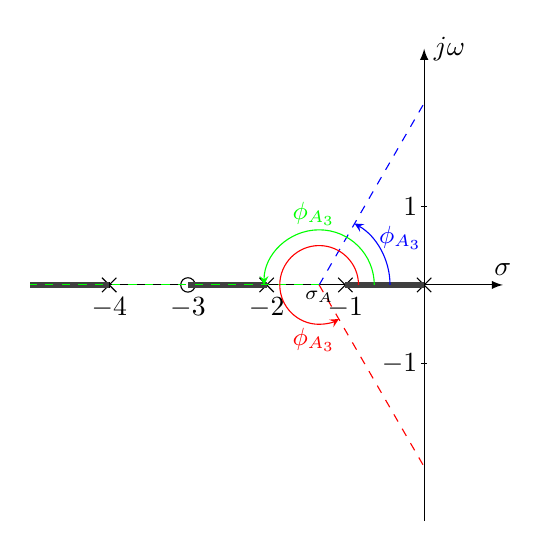
\begin{tikzpicture}
			\rootlocusexample{-3}{3}
			\draw [line width=2pt, darkgray] (0,0) -- (-1,0) {};
			\draw [line width=2pt, darkgray] (-2,0) -- (-3,0) {};
			\draw [line width=2pt, darkgray] (-4,0) -- (-5,0) {};
			\draw [blue, dashed] (-1.3333,0) -- (0,2.3093);
			\draw [green, dashed] (-1.3333,0) -- (-5,0);
			\draw [red, dashed] (-1.3333,0) -- (0,-2.3093);
			\draw [red, -stealth] (-0.83333,0) arc (0:300:0.5);
			\draw [green, -stealth] (-0.63333,0) arc (0:180:0.7);
			\draw [blue, -stealth] (-0.43333,0) arc (0:60:0.9);
			\node [blue] at (-0.3,0.6) {\small $\phi_{A_3}$};
			\node [green] at (-1.4,0.9) {\small $\phi_{A_3}$};
			\node [red]   at (-1.4,-0.7) {\small $\phi_{A_3}$};
			\node [black]   at (-1.33,-0.15) {\scriptsize $\sigma_A$};
		\end{tikzpicture}
\end{figure}	
\end{frame}

\begin{frame}[c]\frametitle{Paso 4: Determinar los puntos de ruptura}
	\begin{itemize}
		\item Ocurren cuando el cambio neto de ángulo ante un pequeño desplazamiento es cero.
		\item El lugar de las raíces se separa en el lugar donde hay multiplicidad de raíces (típicamente 2).
		\item Para determinarlo analíticamente se parte del polinomio característico $1 + KG(s) = 0$. La ecuación se puede reescribir como $K = -1/G(s)$. Se calcula la derivada respecto a $s$ y se iguala a cero:
		\begin{equation*}
			\frac{dK}{ds} = 0
		\end{equation*}
		Finalmente, se calculan las raíces del polinomio resultante.
	\end{itemize}
\end{frame}

\begin{frame}[c]\frametitle{Paso 4: Determinar los puntos de ruptura - Ejemplo}
\vspace*{5mm}
\begin{columns}
	\begin{column}{0.5\textwidth}
	\begin{equation*}
		G(s) = \frac{(s+3)}{s(s+1)(s+2)(s+4)}
	\end{equation*}
	\begin{align*}
		K &= -\frac{1}{G(s)}\\
		&= -\frac{s(s+1)(s+2)(s+4)}{(s+3)}\\
		&= -\frac{s^4+7s^3 + 14s^2 + 8s}{s+3}
	\end{align*}
	\end{column}
	\begin{column}{0.5\textwidth}
	\begin{align*}
		\frac{dK}{ds} &= 0 = -\frac{3s^4 + 26s^3 + 77s^2 + 84s + 24}{(s+3)^2}\\
		0 &= 3s^4 + 26s^3 + 77s^2 + 84s + 24\\
		s &= \{ -3.311 \pm j0.6812, -1.6097, -0.4349 \}
	\end{align*}
	\end{column}
\end{columns}
\vspace*{5mm}
La única raíz que se encuentra dentro del lugar de las raíces es $\sigma_r = -0.4349$.
\end{frame}

\begin{frame}[c]\frametitle{Paso 4: Determinar los puntos de ruptura - Ejemplo}
\begin{figure}
	\begin{tikzpicture}[transform canvas={scale=0.7}]
		\rootlocusexample{-3}{3}
		\draw [line width=2pt, darkgray] (0,0) -- (-1,0) {};
		\draw [line width=2pt, darkgray] (-2,0) -- (-3,0) {};
		\draw [line width=2pt, darkgray] (-4,0) -- (-5,0) {};
		\draw [dashed] (-1.3333,0) -- (1.5,4.9075);
		\draw [dashed] (-1.3333,0) -- (-5,0);
		\draw [dashed] (-1.3333,0) -- (1.5,-4.9075);
		\node at (-0.6,-0.15) {\scriptsize $\sigma_r$};
		\draw (-0.4349,-0.15) -- (-0.4349,0.15);
	\end{tikzpicture}
\end{figure}	
\end{frame}

\begin{frame}[<+->]\frametitle{Paso 5: Determinar el cruce por el eje imaginario}
\begin{itemize}
	\item Se encuentra utilizando el criterio de Routh-Hurwitz.
	\item Se calcula la ganancia crítica $K_{cr}$ para llevar las raíces hasta el eje imaginario.
	\item Se reemplaza la ganancia crítica $K_{cr}$ en el polinomio característico $1 + KG(s) = 0$ y se calculan las raíces.
	\item Se seleccionan las raíces complejas conjugadas (si existen) que tienen parte real igual a cero.
\end{itemize}
\end{frame}

\begin{frame}[c]\frametitle{Paso 5: Determinar el cruce por el eje imaginario - Ejemplo}
\begin{columns}
	\begin{column}{0.5\textwidth}
	\begin{figure}
		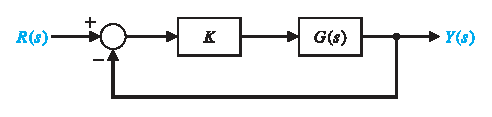
\includegraphics[width=6cm]{images/controlsystem.eps}
		\begin{itemize}
			\item Polinomio característico:	$s^4 + 7 s^3 + 14s^2 + 8s + K(s+3) = 0$
			\item Arreglo de Routh:
			\begin{tabular}{c|ccc}
				$s^4$ & 1 & 14 & $3K$\\
				$s^3$ & 7 & $8+K$ & 0\\
				$s^2$ & $b_1$ & $3K$ & 0\\
				$s^1$ & $c_1$ & 0 & 0\\
				$s^0$ & $3K$ & 0
			\end{tabular}
		\end{itemize}
	\end{figure}
	\end{column}
	\begin{column}{0.5\textwidth}
		\begin{itemize}
			\item Condiciones de estabilidad:
			\begin{align*}
				b_1 &= \frac{90-K}{7} > 0 \Rightarrow K < 90\\
				c_1 &= \frac{-K^2-65K+720}{b_1} > 0 \Rightarrow K_1 < 74.64\ \&\ \\
				&K_2 < 9.65 \Rightarrow K < 9.65
			\end{align*}
			\item Ganancia crítica: $K_{cr} = 9.65$
			\item Reemplazando $K_{cr}$:	$s^4 + 7 s^3 + 14s^2 + 17.65s + 28.95 = 0$ $\Rightarrow$ $\omega_{cr} = \pm 1.588$
		\end{itemize}
	\end{column}
\end{columns}
\end{frame}

\begin{frame}[c]\frametitle{Paso 5: Determinar el cruce por el eje imaginario - Ejemplo}
\begin{figure}
	\begin{tikzpicture}[transform canvas={scale=0.7}]
		\rootlocusexample{-3}{3}
		\draw [line width=2pt, darkgray] (0,0) -- (-1,0) {};
		\draw [line width=2pt, darkgray] (-2,0) -- (-3,0) {};
		\draw [line width=2pt, darkgray] (-4,0) -- (-5,0) {};
		\draw [dashed] (-1.3333,0) -- (1.5,4.9075);
		\draw [dashed] (-1.3333,0) -- (-5,0);
		\draw [dashed] (-1.3333,0) -- (1.5,-4.9075);
		\draw (-0.4349,-0.15) -- (-0.4349,0.15);
		\draw (-0.15,1.588) -- (0.15,1.588);
		\draw (-0.15,-1.588) -- (0.15,-1.588);
		\node at (-0.6,-0.15) {\scriptsize $\sigma_r$};
		\node at (0.4,1.588) {\scriptsize $\omega_{cr}$};
		\node at (0.4,-1.588) {\scriptsize $\omega_{cr}$};
	\end{tikzpicture}
\end{figure}	
\end{frame}

\begin{frame}[c]\frametitle{Paso 6: Finalizar el bosquejo del diagrama - Ejemplo}
\begin{figure}
	\begin{tikzpicture}[transform canvas={scale=0.7}]
		\rootlocusexample{-3}{3}
		\draw [line width=2pt, darkgray] (0,0) -- (-1,0) {};
		\draw [line width=2pt, darkgray] (-2,0) -- (-3,0) {};
		\draw [line width=2pt, darkgray] (-4,0) -- (-5,0) {};
		\draw [dashed] (-1.3333,0) -- (1.5,4.9075);
		\draw [dashed] (-1.3333,0) -- (-5,0);
		\draw [dashed] (-1.3333,0) -- (1.5,-4.9075);
		\draw [line width=2pt, darkgray] plot [smooth] coordinates {(-0.4349,0) (-0.392, 0.43) (-0.281,0.854) (-0.0952,1.36) (0, 1.588) (0.267,2.18) (1.4,4.39)};
		\draw [line width=2pt, darkgray] plot [smooth] coordinates {(-0.4349,0) (-0.392, -0.43) (-0.281,-0.854) (-0.0952,-1.36) (0,-1.588) (0.267,-2.18) (1.4,-4.39)};
		\draw (-0.4349,-0.15) -- (-0.4349,0.15);
		\draw (-0.15,1.588) -- (0.15,1.588);
		\draw (-0.15,-1.588) -- (0.15,-1.588);
		\node at (-0.6,-0.15) {\scriptsize $\sigma_r$};
		\node at (0.4,1.588) {\scriptsize $\omega_{cr}$};
		\node at (0.4,-1.588) {\scriptsize $\omega_{cr}$};
	\end{tikzpicture}
\end{figure}	
\end{frame}

\section{Diseño de Compensadores por LGR - Aproximación de Polos Dominantes}

\begin{frame}[c]\frametitle{Diseño de Compensadores por LGR - Aproximación de Polos Dominantes}
	\begin{itemize}
		\item En el LGR, los polos de lazo cerrado se mueven hacia los ceros de lazo abierto a medida que la ganancia $K$ aumenta.
		\item Lo anterior puede usarse para fijar los polos dominantes deseados del sistema.
		\item El procedimiento puede usarse para diseñar un controlador PID que aproxime los polos dominantes deseados.
	\end{itemize}
\end{frame}

\begin{frame}[c]\frametitle{Diseño de Compensadores por LGR - Aproximación de Polos Dominantes}
	Considere la función de transferencia del controlador PID:
	\begin{equation*}
		G_c(s) = K_p + K_d s + \frac{K_i}{s}
	\end{equation*}
	Reescribiendo el controlador en la forma ideal, donde $K_d = K_p T_d$, $K_i = K_p/T_i$:
	\begin{align*}
		G_c(s) &= K_p \left[1 + T_d s + \frac{1}{T_i s} \right] = K_p \left[ \frac{T_i T_d s^2 + T_i s + 1}{T_i s} \right]\\
		&= \frac{K_p T_i T_d}{s} \left[\frac{s^2 + s/T_d + 1/T_i T_d}{T_i} \right]
	\end{align*}
		
	\begin{align}
		G_c(s) &= \frac{K_p T_d}{s} \left[s^2 + \frac{s}{T_d} + \frac{1}{T_i T_d} \right]\nonumber\\
		&= \frac{K_p T_d}{s} h(s)\label{eq:pid_titd}
	\end{align}
\end{frame}

\begin{frame}[<+->]\frametitle{Diseño de Compensadores por LGR - Aproximación de Polos Dominantes}
\begin{itemize}
	\item El diagrama de bloques del sistema se puede organizar como:
	\begin{figure}	
	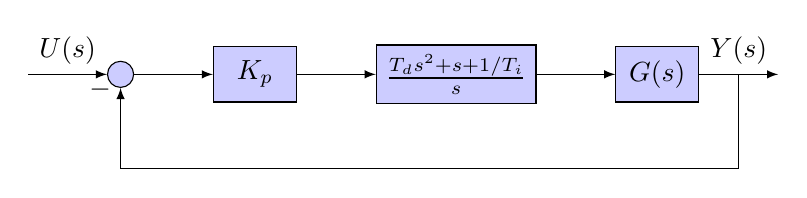
\begin{tikzpicture}[auto, node distance=1cm,>=latex]
	  \node [input, name=input] {};
	  \node [sum, right=of input] (sum) {};
	  \node [block, right=of sum] (gain) {$K_p$};
	  \node [block, right=of gain] (controller) {$\frac{T_d s^2 + s + 1/T_i}{s}$};
	  \node [block, right=of controller] (plant) {$G(s)$};
	  \node [output, right=of plant] (output) {};
	  \draw [draw,->] (input) -- node {$U(s)$} (sum);
	  \draw [->] (sum) -- node {} (gain);
	  \draw [->] (gain) -- node {} (controller);
	  \draw [->] (controller) -- node {} (plant);
	  \draw [->] (plant) -- node [name=y] {$Y(s)$}(output);
	  \draw [->] (y) -- ++ (0,-1.5) -| node [pos=0.99] {$-$} (sum);
	\end{tikzpicture}
	\end{figure}
	\item Combinando el bloque que depende de $T_i$, $T_d$ con la planta:
	\begin{figure}	
	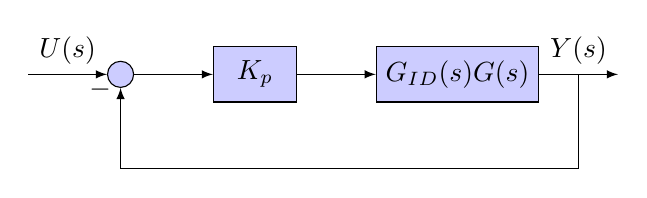
\begin{tikzpicture}[auto, node distance=1cm,>=latex]
	  \node [input, name=input] {};
	  \node [sum, right=of input] (sum) {};
	  \node [block, right=of sum] (gain) {$K_p$};
	  \node [block, right=of gain] (plant) {$G_{ID}(s)G(s)$};
	  \node [output, right=of plant] (output) {};
	  \draw [draw,->] (input) -- node {$U(s)$} (sum);
	  \draw [->] (sum) -- node {} (gain);
	  \draw [->] (gain) -- node {} (plant);
	  \draw [->] (plant) -- node [name=y] {$Y(s)$}(output);
	  \draw [->] (y) -- ++ (0,-1.5) -| node [pos=0.99] {$-$} (sum);
	\end{tikzpicture}
	\end{figure}
	\item Usando $T_i$, $T_d$ es posible fijar los ceros de lazo abierto del sistema $G_{ID}(s)G(s)$.
	\item Usando $K_p$, es posible ubicar los polos de lazo cerrado cerca de los ceros de lazo abierto, aproximando el desempeño deseado.
\end{itemize}
\end{frame}

\begin{frame}[c]\frametitle{Procedimiento de Diseño}
	\begin{enumerate}
		\item A partir de los requerimientos de desempeño, encontrar un polinomio deseado $q_{des}(s)$ para el sistema en lazo cerrado. Calcular la ubicación de los polos de dicho polinomio.
		\item Comparar el polinomio deseado con el polinomio $h(s)$ en la Ec.\eqref{eq:pid_titd}. Resolver el sistema de ecuaciones para hallar $T_i$, $T_d$.
		\item Sustituir los valores $T_i$, $T_d$ en $G_{ID}(s)$. Dibujar el lugar de las raíces para el sistema $G_{ID}(s)G(s)$.
		\item Encontrar una ganancia $K_p$ tal que los polos de lazo cerrado se aproximen a los ceros de lazo abierto.
		\item Reemplazar $K_p$, $T_i$, $T_d$ en $G_c(s)$. Simular el sistema y verificar el desempeño.
	\end{enumerate}
\end{frame}

\begin{frame}[c]\frametitle{Diseño de Compensadores por LGR - Ejemplo}
	Considere el sistema:
	\begin{equation*}
		G(s) = \frac{0.8}{(30s+1)(13s+1)(3s+1)}
	\end{equation*}
	Se desea un controlador PID sintonizado usando el LGR tal que tenga un sobrepico $PO \leq 15\%$ y tiempo de establecimiento $T_s = 100$ s con $e_{ss} = 0$. 
\end{frame}

\begin{frame}[c]\frametitle{Diseño de Compensadores por LGR - Ejemplo}
	Con el sobrepico se calcula el valor de $\zeta$:
	\begin{equation*}
		e^{-\pi \zeta/\sqrt{1-\zeta^2}} = 0.15 \hspace*{2mm} \Rightarrow \hspace*{2mm} \zeta = 0.5165
	\end{equation*}
	Con el tiempo de estabilización $T_s$ y el valor de $\zeta$ encontrado, se obtiene el valor de $\omega_n$:
	\begin{align*}
		T_s = \frac{4}{\zeta \omega_n} \hspace*{2mm} \Rightarrow \vspace*{2mm} \omega_n = 0.0774
	\end{align*}
	Entonces, el polinomio deseado es:
	\begin{equation*}
		q_{des} = s^2 + 2\zeta\omega_n s + \omega_n^2 = s^2 + 0.08 s + 0.006
	\end{equation*}
\end{frame}

\begin{frame}[c]\frametitle{Diseño de Compensadores por LGR - Ejemplo}
	Se compara el polinomio deseado con el polinomio que define los ceros del controlador PID:
	\begin{equation*}
		h(s) = s^2 + \frac{s}{T_d} + \frac{1}{T_i T_d}		
	\end{equation*}
	Entonces, se obtienen las siguientes ecuaciones:
	\begin{equation*}
		\frac{1}{T_d} = 0.080, \hspace*{3mm} \frac{1}{T_i T_d} = 0.0059
	\end{equation*}
	\begin{equation*}
		T_i = 13.3608, \vspace*{3mm} T_d = 12.50
	\end{equation*}
\end{frame}

\begin{frame}[c]\frametitle{Diseño de Compensadores por LGR - Ejemplo}
\begin{columns}
	\begin{column}{0.5\textwidth}
	\begin{itemize}
		\item Usando la función \texttt{rlocus} de Matlab, se obtiene el lugar de las raíces.
		\item Note que los dos polos reales ubicados en $s = 0$ y $s = 0.0333$ colisionan y se convierten en un par de polos complejos conjugados que tienden hacia los ceros ubicados en $-0.04 \pm j0.0662$ a medida que $K_p \rightarrow \infty$.
	\end{itemize}
	\end{column}
	\begin{column}{0.5\textwidth}
	\begin{figure}
		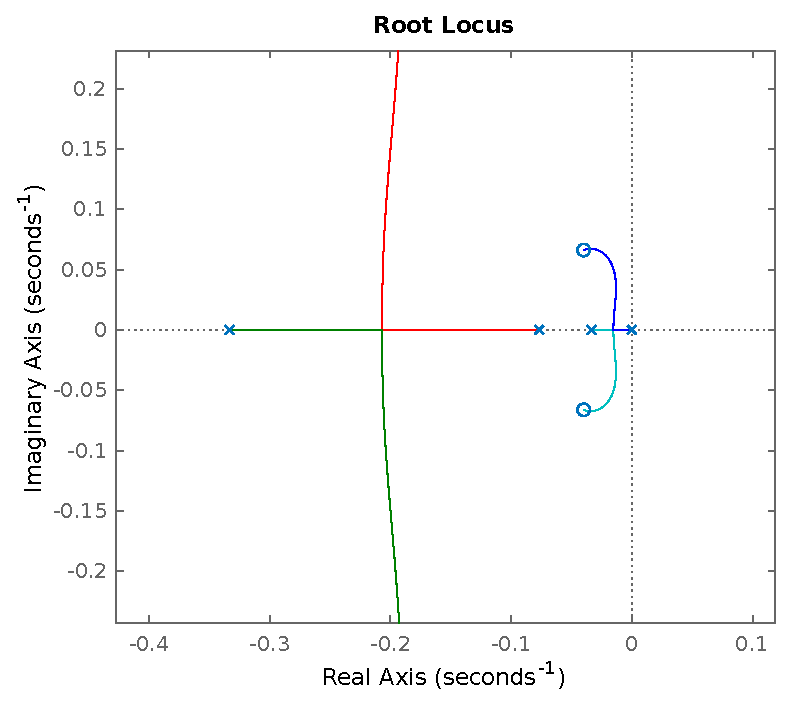
\includegraphics[width=7cm]{images/LGR_example.eps}
	\end{figure}
	\end{column}
\end{columns}
\end{frame}

\begin{frame}[c]\frametitle{Diseño de Compensadores por LGR - Ejemplo}
\begin{columns}
	\begin{column}{0.5\textwidth}
	\small
	\begin{itemize}
		\item Ahora hay que encontrar una ganancia $K_p$ para aproximar la ubicación de los polos dominantes deseados. Para hacerlo se puede usar la herramienta \texttt{rltool}.
		\item Ajustando la ganancia en la herramienta \texttt{rltool} se encuentra que con $K_p = 131.01$, los polos dominantes resultantes se encuentran ubicados en $s = -0.0296 \pm j0.0667$.
		\item Con ésta ubicación se obtiene la siguiente respuesta paso:
	\end{itemize}	
	\end{column}
	\begin{column}{0.5\textwidth}
	\small
	\begin{figure}
		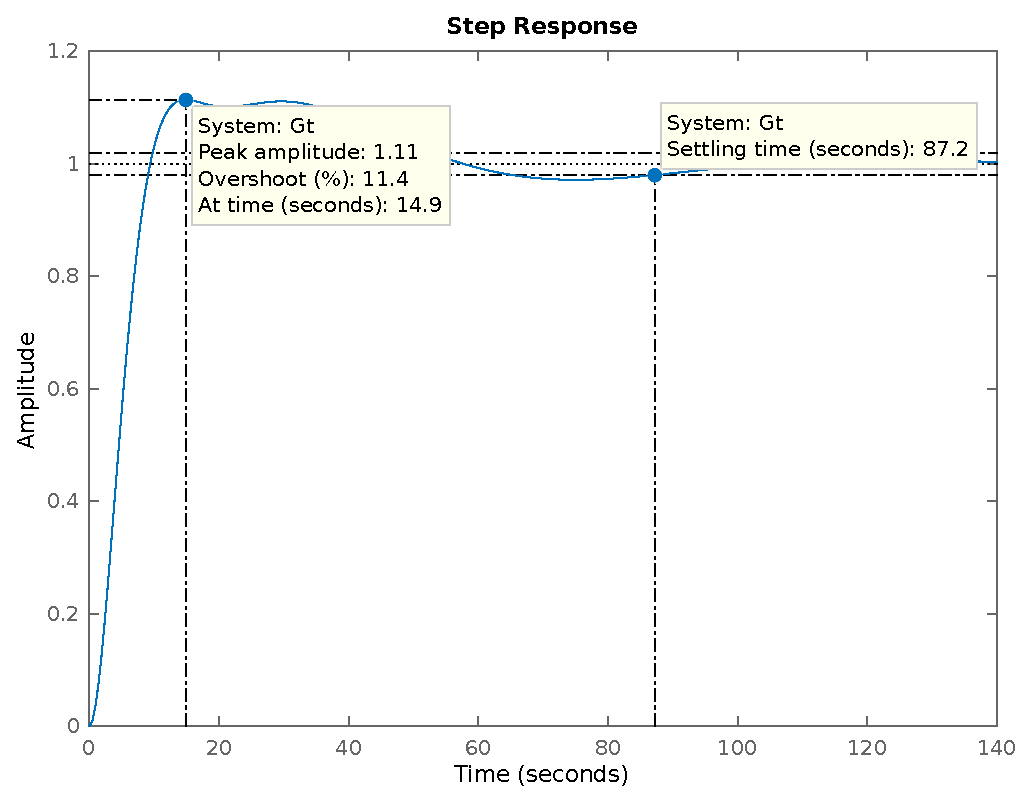
\includegraphics[width=7cm]{images/LGR_examaple_step.eps}
	\end{figure}
	\centering
	\textbf{Si se satisfacen los requerimientos!}
	\end{column}
\end{columns}
\end{frame}

\begin{frame}[c]\frametitle{Taller}
\begin{enumerate}
	\item Considere la función de transferencia de lazo abierto
	\begin{equation*}
		KG(s) = \frac{K}{s(s+2)(s^2+4s+5)}
	\end{equation*}
	\begin{itemize}
		\item Realice un bosquejo del lugar de las raíces. Verifique el resultado usando \texttt{rlocus}.
		\item Calcule la ubicación de los polos dominantes cuando $K = 6.5$.
		\item Para los polos dominantes encontrados, calcule el tiempo de establecimiento y el sobrepico para una entrada paso. Verifique los resultados con una simulación.
	\end{itemize}
	\seti
\end{enumerate}
\end{frame}

\begin{frame}[c]\frametitle{Taller}
	\begin{enumerate}
		\conti
		\item Un sistema de control tiene la siguiente función de transferencia de lazo abierto:
		\begin{equation*}
			KG(s) = \frac{K(s+2.5)}{(s^2+2s+2)(s^2+4s+5)}
		\end{equation*}
		\begin{itemize}
			\item Realice un bosquejo del lugar de las raíces. Verifique el resultado usando \texttt{rlocus}.
			\item Encuentre la ganancia $K$ que resulta en polos dominantes con un factor de amortiguamiento de 0.707.
			\item Encuentre el porcentaje de sobrepico y tiempo de pico para la ganancia $K$ calculada. Verifique el resultado usando una simulación.
		\end{itemize}
		\seti
	\end{enumerate}
\end{frame}

\begin{frame}[c]\frametitle{Taller}
	\begin{enumerate}
		\conti
		\item Un sistema de control tiene la siguiente función de transferencia de lazo abierto:
		\begin{equation*}
			KG(s) = \frac{K(s+1)}{s(s-1)(s+4)}
		\end{equation*}
		\begin{itemize}
			\item Determine el rango de estabilidad de $K$.
			\item Realice un bosquejo del lugar de las raíces. Verifique el resultado usando \texttt{rlocus}.
			\item Determine el máximo valor de $\zeta$ de las raíces complejas estables.
		\end{itemize}
		\seti
	\end{enumerate}
\end{frame}

\begin{frame}[c]\frametitle{Taller}
	\begin{enumerate}
		\conti
		\item Considere la planta caracterizada por la función de transferencia
		\begin{equation*}
			G(s) = \frac{(s+3)}{(s-1)(s+2)(s+5)}
		\end{equation*}
		Se desea diseñar un sistema de control que cumpla con las siguientes especificaciones ante una entrada paso unitaria:
		\begin{itemize}
			\item Porcentaje de sobrebico: 10\%.
			\item Tiempo de establecimiento: 10 s.
			\item Error de estado estacionario: 0.
		\end{itemize}
		Diseñe un controlador PID usando el lugar de las raíces por el método de aproximación de polos dominantes. Verifique el resultado usando simulaciones.
	\end{enumerate}
\end{frame}

\end{document}